\chapter{NIST Special Publication 800-90B}
\label{chap:NIST800-90B}
\section{General}

Topic of this thesis is an analysis of a Linux Random Number Generator's outcome delivered to kernel consumers, as introduced in \ref{sub:get-rnd-int-long}. Verification and estimation of entropy is 
a very difficult task, since there is no explicit definition for randomness. Hence, for a series of values generated by an RNG, randomness i.e. a sufficient degree of entropy is admitted, if the absence of any discernible pattern within a generated record can be diagnosed.
To assess the outcome and reliability of random number generating devices or implementations, several frameworks have been published, providing recommendations regarding the solid construction and validation of PRNG and TRNG sources. These also encompass a set of statistical tests and guidance how to conduct a profound verification (see \cite{robert2006dieharder, rukhin2010nist, turan2018nist}).
The National Institute of Standards and Technology (NIST) publishes a series of documents that describe U.S. federal government computer security policies, procedures and guidelines called NIST 800 series (see \cite[]{nist800pub}). To implement the analysis of this thesis, two Special Publications on the subject of validation and assessment of entropy and random number generation has been chosen:

\begin{table}[H]
	\centering
	\label{tab:nist800sps}
	\begin{tabular}{lll}\\ \hline 
		Number & Title & Release Date \\ \hline \hline 
		800-90B & \makecell[l]{Recommendation for the Entropy Sources Used for\\Random Bit Generation} & 1/10/2018 \\ \hline 
		800-22 Rev. 1a & \makecell[l]{A Statistical Test Suite for Random and Pseudorandom\\Number Generators for Cryptographic Applications} & 4/30/2010 \\ \hline 
	\end{tabular}
	\caption{Applied NIST Special Publications of the 800 Series (Status Final)}
\end{table} 


"Recommendation for the Entropy Sources Used for Random Bit Generation"

have been chosen, 
%\citetalias{turan2018nist}

%rukhin2010nist

For this analysis, a framework based on 'Recommendation for the Entropy Sources Used for Random Bit Generation, NIST Special Publication 800- 90B' \cite{turan2018nist} has been chosen, able to deliver
usable guidance that will give conservative estimates on the amount of entropy in an entropy
source \cite{turan2015random}. The final version of the framework has been published in january 2018 and thus is very up to date. Beside that this decision has been met, since not just the outcome of and RNG can be assessed but also it's input. As mentioned in \ref{sec:int-rnd}, the Linux RNG executed on a Xen virtualized machine is not able to obtain noise from most designated sources. In fact, interrupt noise is the only input delivered during the initialization phase. Hence, to achieve a comprehensive analysis, an assessment of this input is considered to be required.\\
'NIST Special Publication (SP) 800-90' (a series consisting of three documents) specifies how to design an test 

 is all about
generating random numbers for cryptography. In SP 800-90, this is a two-stage process: first, an
entropy source provides an impossible-to-guess seed. Then, a deterministic cryptographic
algorithm (called a DRBG--deterministic random bit generator--in SP 800-90) expands the seed
into a long sequence of values that may be safely used for keys, IVs, nonces, etc.
\cite{turan2015random}.



 When assessing entropy by the second part of the series, 'NIST Special Publication 800-90B' (in the following referred to as NSP800-90B), an estimation can be achieved via 
two different tracks. Depending on an assumption regarding an entropy source, which has to be substantiated, the IID i.e. the Non-IID track should be used to analyze assumed random input 
\cite{turan2018nist}. The outcome of an analysis is an estimation of entropy, ascertained by statistical tests expressed in \textit{bits of entropy}. In the following sections, an introduction to these procedures, required to comprehend the results in TODO[Evaludation] is given.



%-----------------------------------------------
%NIST Special Publication (SP) 800-90 (a series consisting of three documents) is all about
%generating random numbers for cryptography. In SP 800-90, this is a two-stage process: first, an
%entropy source provides an impossible-to-guess seed. Then, a deterministic cryptographic
%algorithm (called a DRBG--deterministic random bit generator--in SP 800-90) expands the seed
%into a long sequence of values that may be safely used for keys, IVs, nonces, etc.
%\cite{turan2015random}

\section{Definitions \& Terminology}

\subsection{Distinction: Noise / Entropy / Randomness}
In literature, terms describing the in- and output of RNGs are sometimes used in an alternating and partially confusing manner. For this thesis, the following terminology will be used:

\begin{itemize}
	\item \textbf{Entropy} Entropy is a of a variable or value describing a certain degree of unpredictability. The referred NIST 800 Special Publications use the term \textit{Entropy Source} for \textit{Noise Source} as well as \textit{Randomness Source}, which is correct but sometimes confusing.
	\item \textbf{Noise} Noise is the raw input passed to an RNG. The noise sources of the Linux RNG are described in \ref{sec:inp-src-lprng}. While there might be a wide range, in general, noise is not assumed to provide a cryptographic safe degree of entropy. 
	\item \textbf{Randomness} The outcome of an RNG. The Linux RNG generates random numbers on basis of noise being prepared by pre-processors and conditioning components. This output is assumed to provide a cryptographic safe degree of entropy.  
	\item \textbf{RBG/RNG} NIST 800 uses the more generalizing term \textit{RBG (Random Bit Generator)} instead of \textit{RNG (Random Number Generator)}. Since this thesis relates to Linux x86 Kernel where random numbers are always obtained and applied on at least byte level \textit{RNG} will used.
\end{itemize}

\subsection{The Definition of Entropy}
In Information theory, for a set of information units, entropy in generall describes the level of disorder i.e. the unpredicatbility of each single unit's state at a given alphabet. Various formal defintions of entropy exist \cite{hagerty2012entropy}, while the definition of Shannon (see \ref{fig:form-entropy-shan}) is quite common for a binary alphabet. 

\begin{figure}[H]
	\begin{align*}
	\displaystyle H(X) := \sum_{s \in {0,1}} I(p_s) p_s = \sum_{s \in {0,1}} -\lg_2 \frac{1}{p_s} p_s && \text{$p_s$ = P(X=s)}
	\end{align*}
	\caption{Formal definiton of entropy by Shannon for a binary alphabet}
	\label{fig:form-entropy-shan}
\end{figure}
According to Shannon, entropy is defined as the product of self-information \textit{I} multiplied by the expected value. For a binary alphabet, it can be measured in unit bits. 



\section{NIST Special Publication 800-90 B}

The NIST Special Publication (SP) 800-90 series of recommendations provides 
guidance on the validation and construction of Pseudo- and Non-deterministic Random Number Generators that can be used for cryptographic secure applications. The recommendation specifies how to design and test noise sources that are be used as input for RNGs. The series consist of three parts. NSP800-90A and NSP800-90C refer to the construction of RNG mechanisms, while NSP800-90B addresses the analysis and validation of noise sources. A noise source that conforms to this recommendation can be used by RNGs to produce a sequence of random values \cite{rukhin2010nist}.

\subsection{Min-Entropy}

\begin{equation}
	A = \{x_1, x_2, x_3, ..., x_k\}
	\label{eq:min-ent-A}
\end{equation}
\begin{equation}
	Pr(X=x_i) = p_i 
	\Domain{i=\{1,...,k\}}
\end{equation}
\begin{equation}
	H = \underset{1\leq i\leq k}{\mathrm{min}}(-\log_2p_i) = -\log_2 \underset{1\leq i\leq k}{\mathrm{max}}p_i
\end{equation}



\begin{figure}[H]
	\label{fig:entropy-est-strategy}
	\centering
	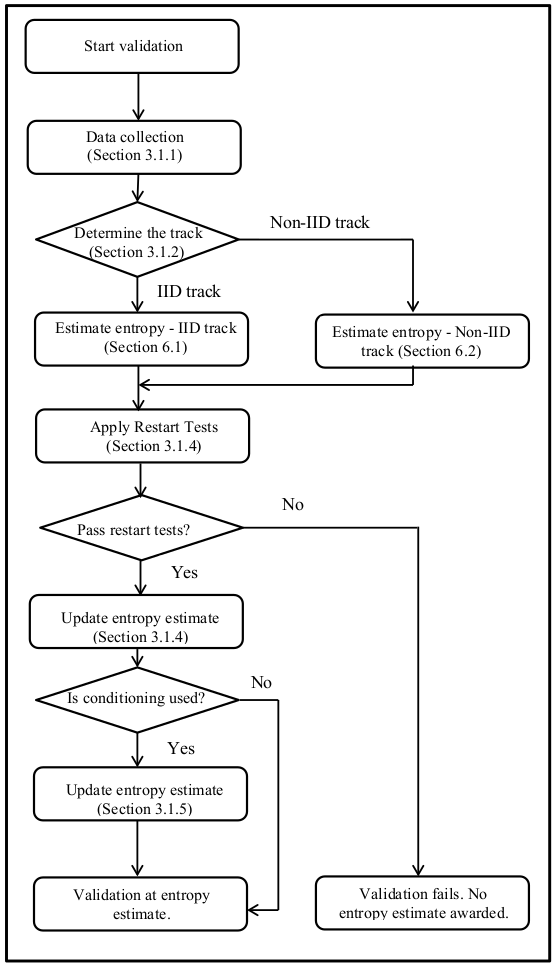
\includegraphics[scale=0.6]{img/nsp800-90b-entropy-est-strategy.png}
	\caption{Entropy Estimation Strategy according to NIST SP 800-90B (from \cite{turan2018nist}, references illustrated refer to the document)}
\end{figure}




